
\chapter{Introdução}

Este projeto intitulado \textit{Install \& Go}, refere-se a uma aplicação para \textit{smartphone} direcionada a todos os clientes e 
técnicos Motorline, com o propósito de agilizar todo o processo de resolução de problemas e de acesso 
aos produtos. Para alcançar estes objetivos, a aplicação conta com um catálogo para todos os utilizadores 
e também com um fórum para os clientes e técnicos Motorline.

No início de estágio foi indicado pelo supervisor da empresa a subdivisão do projeto em duas grandes componentes. Também este projeto foi desenvolvido com uma colega que ficou encarregue de desenvolver o \textit{frontend} da componente do catálogo. Já o desenvolvimento completo do \textit{backend}, aquisição do catálogo de produtos do \textit{website} da empresa e o \textit{frontend} para o fórum, gestão de utilizadores e autenticação ficaram a cargo do autor deste documento.

O fórum da aplicação é uma plataforma que permite aos clientes e técnicos criar tópicos para realizar questões e/ou expor problemas para a comunidade. Estes tópicos podem ser comentados, onde também é possível realizar uma comunicação.

O suporte \textit{backend} da aplicação foi realizado através de um conjunto de serviços, sendo inicialmente apenas necessário para fórum. Contudo, foi posteriormente acrescentado suporte para o catálogo de produtos.


\section{Objetivos}
A plataforma do fórum da aplicação deverá permitir que a comunidade partilhe os seus tópicos. Para isso, o utilizador necessitará conseguir criar estes com a indicação do problema e uma descrição do mesmo, com a possibilidade de anexar imagens, assim como referenciar o produto, para facilitar a identificação e resolução do problema.

A comunidade deverá também ter a possibilidade de comentar os tópicos e comunicar nesta secção. O responsável pelo tópico necessitará ter a possibilidade de o colocar em privado caso tenha como objetivo que apenas técnicos Motorline respondam ao mesmo. Este também deverá ter a seu dispor a possibilidade de indicar quando a tópico estiver finalizado e qual a melhor resposta que obteve. Os utilizadores deverão também conseguir gostar de tópicos e comentários para destacar os mesmos perante a restante comunidade.

A comunidade deverá conseguir ver os tópicos em destaque, os mais recentes, os seus tópicos, os que não estão finalizados e os técnicos Motorline necessitarão de conseguir ver os tópicos privados existentes. A comunidade deverá ter a possibilidade de pesquisar por tópicos com assuntos específicos, pesquisa por nome e por produto. Para filtragem de pesquisa a comunidade deverá também conseguir selecionar o tipo de tópico.

\section{Contexto}
O projeto foi desenvolvido na empresa Motorline Eletrocelos S.A daqui em diante designada Motorline, esta empresa é especializada na produção e comercialização de automatismos para portas e portões, sistemas de controlo de acessos, sistemas de segurança, entre outros produtos relacionados com o setor da automação.

Este projeto vem por este meio resolver o problema de comunicação com o cliente, que atualmente para solucionar as suas questões tem de contactar a assistência técnica que por vezes pode estar sobrecarregada, pelo que deverão preencher um formulário para expor a sua questão.

Com esta solução os clientes e técnicos Motorline poderão procurar ou expor os seus problemas com a comunidade onde têm a possibilidade de ser respondidos, o que torna o processo de resolução de problemas mais ágil.



\section{Estrutura do documento}

Este documento contém a descrição de todo o processo de engenharia de \textit{software}, desenvolvimento e pensamento sobre o problema em mãos, sendo estes pontos divididos sobre diversos tópicos:
\begin{enumerate}
  \item Estado da Arte, onde é abordado as ferramentas utilizadas e tecnologias exploradas.
  \item Análise e especificação, onde é abordado o estudo das soluções existentes, descrito o modelo de negócio e apresentada toda a engenharia de \textit{software}
  \item Trabalho desenvolvido, onde é descrito todo o processo de desenvolvimento do projeto.
  \item Análise de resultados, onde é discutido os resultados obtidos.
  \item Conclusão e trabalho futuro, onde é abordada a conclusão sobre o projeto e também futuras implementações que poderiam ser realizadas.
\end{enumerate}


\newpage

\section{Planificação do trabalho}\label{sec:planificacao trabalho}

Para obter uma visão geral do projeto e uma previsão de finalização foi realizada uma planificação expectável de tarefas. Encontra-se no documento de anexos, no anexo 1, uma versão mais detalhada da Figura~\ref*{fig:1}.

\begin{figure}[htb]
  \centering
  
  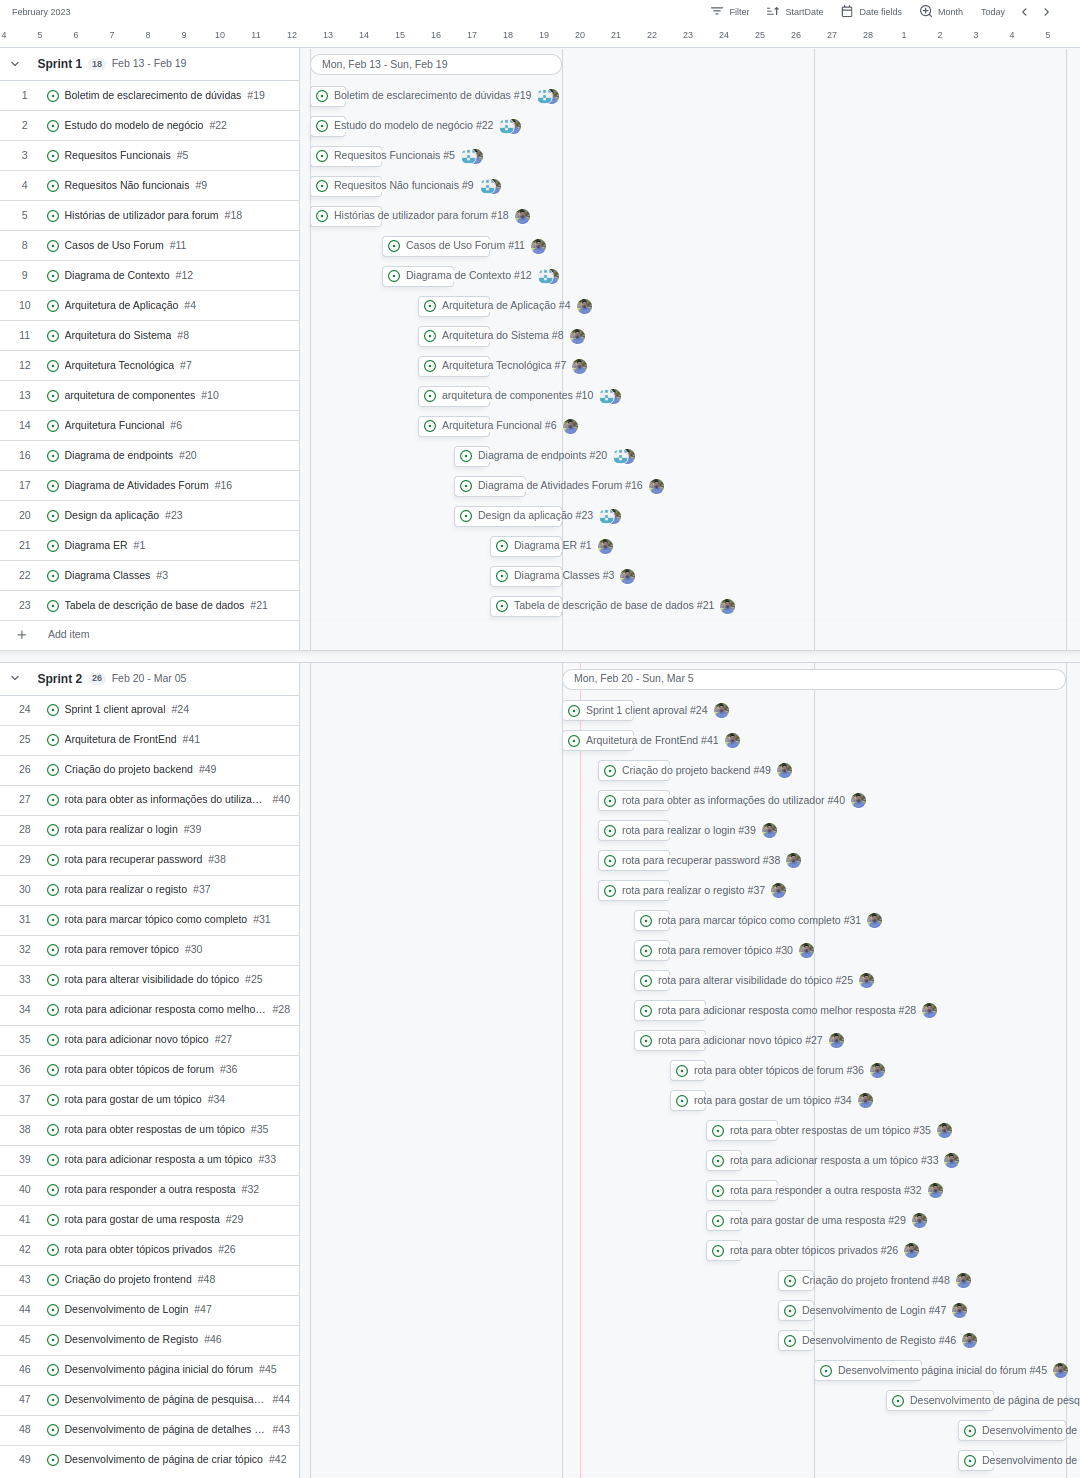
\includegraphics[width=0.83\textwidth]{images/etapa1_sprint_planning.png}
  \caption{Planificação de \textit{sprints}}
  \label{fig:1}
\end{figure}
